% Options for packages loaded elsewhere
\PassOptionsToPackage{unicode}{hyperref}
\PassOptionsToPackage{hyphens}{url}
%
\documentclass[
  10pt,
  b5paper,
  oneside]{book}
\usepackage{amsmath,amssymb}
\usepackage{lmodern}
\usepackage{ifxetex,ifluatex}
\ifnum 0\ifxetex 1\fi\ifluatex 1\fi=0 % if pdftex
  \usepackage[T1]{fontenc}
  \usepackage[utf8]{inputenc}
  \usepackage{textcomp} % provide euro and other symbols
\else % if luatex or xetex
  \usepackage{unicode-math}
  \defaultfontfeatures{Scale=MatchLowercase}
  \defaultfontfeatures[\rmfamily]{Ligatures=TeX,Scale=1}
\fi
% Use upquote if available, for straight quotes in verbatim environments
\IfFileExists{upquote.sty}{\usepackage{upquote}}{}
\IfFileExists{microtype.sty}{% use microtype if available
  \usepackage[]{microtype}
  \UseMicrotypeSet[protrusion]{basicmath} % disable protrusion for tt fonts
}{}
\makeatletter
\@ifundefined{KOMAClassName}{% if non-KOMA class
  \IfFileExists{parskip.sty}{%
    \usepackage{parskip}
  }{% else
    \setlength{\parindent}{0pt}
    \setlength{\parskip}{6pt plus 2pt minus 1pt}}
}{% if KOMA class
  \KOMAoptions{parskip=half}}
\makeatother
\usepackage{xcolor}
\IfFileExists{xurl.sty}{\usepackage{xurl}}{} % add URL line breaks if available
\IfFileExists{bookmark.sty}{\usepackage{bookmark}}{\usepackage{hyperref}}
\hypersetup{
  pdftitle={Country guidelines and specifications for Digital Soil Mapping},
  pdfauthor={GSP Secretariat and ITPS},
  hidelinks,
  pdfcreator={LaTeX via pandoc}}
\urlstyle{same} % disable monospaced font for URLs
\usepackage{color}
\usepackage{fancyvrb}
\newcommand{\VerbBar}{|}
\newcommand{\VERB}{\Verb[commandchars=\\\{\}]}
\DefineVerbatimEnvironment{Highlighting}{Verbatim}{commandchars=\\\{\}}
% Add ',fontsize=\small' for more characters per line
\usepackage{framed}
\definecolor{shadecolor}{RGB}{248,248,248}
\newenvironment{Shaded}{\begin{snugshade}}{\end{snugshade}}
\newcommand{\AlertTok}[1]{\textcolor[rgb]{0.94,0.16,0.16}{#1}}
\newcommand{\AnnotationTok}[1]{\textcolor[rgb]{0.56,0.35,0.01}{\textbf{\textit{#1}}}}
\newcommand{\AttributeTok}[1]{\textcolor[rgb]{0.77,0.63,0.00}{#1}}
\newcommand{\BaseNTok}[1]{\textcolor[rgb]{0.00,0.00,0.81}{#1}}
\newcommand{\BuiltInTok}[1]{#1}
\newcommand{\CharTok}[1]{\textcolor[rgb]{0.31,0.60,0.02}{#1}}
\newcommand{\CommentTok}[1]{\textcolor[rgb]{0.56,0.35,0.01}{\textit{#1}}}
\newcommand{\CommentVarTok}[1]{\textcolor[rgb]{0.56,0.35,0.01}{\textbf{\textit{#1}}}}
\newcommand{\ConstantTok}[1]{\textcolor[rgb]{0.00,0.00,0.00}{#1}}
\newcommand{\ControlFlowTok}[1]{\textcolor[rgb]{0.13,0.29,0.53}{\textbf{#1}}}
\newcommand{\DataTypeTok}[1]{\textcolor[rgb]{0.13,0.29,0.53}{#1}}
\newcommand{\DecValTok}[1]{\textcolor[rgb]{0.00,0.00,0.81}{#1}}
\newcommand{\DocumentationTok}[1]{\textcolor[rgb]{0.56,0.35,0.01}{\textbf{\textit{#1}}}}
\newcommand{\ErrorTok}[1]{\textcolor[rgb]{0.64,0.00,0.00}{\textbf{#1}}}
\newcommand{\ExtensionTok}[1]{#1}
\newcommand{\FloatTok}[1]{\textcolor[rgb]{0.00,0.00,0.81}{#1}}
\newcommand{\FunctionTok}[1]{\textcolor[rgb]{0.00,0.00,0.00}{#1}}
\newcommand{\ImportTok}[1]{#1}
\newcommand{\InformationTok}[1]{\textcolor[rgb]{0.56,0.35,0.01}{\textbf{\textit{#1}}}}
\newcommand{\KeywordTok}[1]{\textcolor[rgb]{0.13,0.29,0.53}{\textbf{#1}}}
\newcommand{\NormalTok}[1]{#1}
\newcommand{\OperatorTok}[1]{\textcolor[rgb]{0.81,0.36,0.00}{\textbf{#1}}}
\newcommand{\OtherTok}[1]{\textcolor[rgb]{0.56,0.35,0.01}{#1}}
\newcommand{\PreprocessorTok}[1]{\textcolor[rgb]{0.56,0.35,0.01}{\textit{#1}}}
\newcommand{\RegionMarkerTok}[1]{#1}
\newcommand{\SpecialCharTok}[1]{\textcolor[rgb]{0.00,0.00,0.00}{#1}}
\newcommand{\SpecialStringTok}[1]{\textcolor[rgb]{0.31,0.60,0.02}{#1}}
\newcommand{\StringTok}[1]{\textcolor[rgb]{0.31,0.60,0.02}{#1}}
\newcommand{\VariableTok}[1]{\textcolor[rgb]{0.00,0.00,0.00}{#1}}
\newcommand{\VerbatimStringTok}[1]{\textcolor[rgb]{0.31,0.60,0.02}{#1}}
\newcommand{\WarningTok}[1]{\textcolor[rgb]{0.56,0.35,0.01}{\textbf{\textit{#1}}}}
\usepackage{longtable,booktabs,array}
\usepackage{calc} % for calculating minipage widths
% Correct order of tables after \paragraph or \subparagraph
\usepackage{etoolbox}
\makeatletter
\patchcmd\longtable{\par}{\if@noskipsec\mbox{}\fi\par}{}{}
\makeatother
% Allow footnotes in longtable head/foot
\IfFileExists{footnotehyper.sty}{\usepackage{footnotehyper}}{\usepackage{footnote}}
\makesavenoteenv{longtable}
\usepackage{graphicx}
\makeatletter
\def\maxwidth{\ifdim\Gin@nat@width>\linewidth\linewidth\else\Gin@nat@width\fi}
\def\maxheight{\ifdim\Gin@nat@height>\textheight\textheight\else\Gin@nat@height\fi}
\makeatother
% Scale images if necessary, so that they will not overflow the page
% margins by default, and it is still possible to overwrite the defaults
% using explicit options in \includegraphics[width, height, ...]{}
\setkeys{Gin}{width=\maxwidth,height=\maxheight,keepaspectratio}
% Set default figure placement to htbp
\makeatletter
\def\fps@figure{htbp}
\makeatother
\setlength{\emergencystretch}{3em} % prevent overfull lines
\providecommand{\tightlist}{%
  \setlength{\itemsep}{0pt}\setlength{\parskip}{0pt}}
\setcounter{secnumdepth}{5}
\usepackage{booktabs}
\usepackage{amsthm}
\makeatletter
\let\stdl@chapter\l@chapter
\renewcommand*{\l@chapter}[2]{%
  \stdl@chapter{\textcolor{astral}{#1}}{\textcolor{astral}{#2}}}

\def\thm@space@setup{%
  \thm@preskip=5cm
  \thm@postskip=\thm@preskip

}

\usepackage{afterpage}

\newcommand\blankpage{%
    \null
    \thispagestyle{empty}%
    \addtocounter{page}{-1}%
    \newpage}

\usepackage{amssymb}
\usepackage{amsmath}
%\pagestyle{plain} % default for report

\usepackage{etoolbox}
\makeatletter
\patchcmd{\@makechapterhead}{50\p@}{-24pt}{}{}
\patchcmd{\@makeschapterhead}{50\p@}{-24pt}{}{}
\makeatother

\makeatother
\usepackage{sectsty}

\definecolor{astral}{RGB}{153, 61, 15}
\allsectionsfont{\sffamily\color{astral}}

\hypersetup{
    colorlinks=true,
    linkcolor=astral,
    filecolor=astral,
    urlcolor=astral,
    citecolor=astral
}

\usepackage{fancyhdr}
\usepackage{pdfpages}

\renewcommand{\headrulewidth}{0.5pt}
\renewcommand{\headrule}{\hbox to\headwidth{\color{astral}\leaders\hrule height \headrulewidth\hfill}}


\setlength{\headheight}{5pt}

\fancyhf{}
\fancyhead[EL]{\nouppercase\leftmark}
\fancyhead[OR]{\nouppercase\rightmark}
\fancyhead[ER,OL]{\thepage}

\usepackage{multicol}

\usepackage{longtable}
\usepackage{array}
\usepackage{multirow}
\usepackage{wrapfig}
\usepackage{float}
\usepackage{colortbl}
\usepackage{pdflscape}
\usepackage{tabu}
\usepackage{threeparttable}
\usepackage[normalem]{ulem}
% empty pages betwen chapters
\usepackage{emptypage}

\makeatletter
\makeatother

\renewcommand{\listfigurename}{Figures}
\renewcommand{\listtablename}{Tables}

\usepackage[sectionbib]{chapterbib}

%% List of Abbreviations
\usepackage{nomencl}
\makenomenclature
\renewcommand{\nomname}{Acronyms}
%% to update run makeindex on docs folder and move results to / folder
%% see nomencl manual
%% e.g. makeindex SOCMapping.nlo -s nomencl.ist -o SOCMapping.nls

%% index
\usepackage{imakeidx}
\makeindex

\usepackage{xspace}

% no title page
\AtBeginDocument{\let\maketitle\relax}
\AtBeginDocument{\renewcommand{\chaptername}{Chapter}}
\usepackage{titling}
\usepackage{natbib}
\usepackage{pdfpages}
\usepackage{fancyhdr}
\usepackage{booktabs}
\usepackage{longtable}
\usepackage{subfig}
\usepackage{array}
\usepackage{amsmath}
\usepackage{multirow}
\usepackage{wrapfig}
\usepackage{bookmark}
\usepackage[utf8]{inputenc}
\usepackage{float}
\usepackage{colortbl}
\usepackage{pdflscape}
\usepackage{tabu}
\usepackage{threeparttable}
\usepackage{threeparttablex}
\usepackage[normalem]{ulem}
\usepackage{makecell}
\usepackage{xcolor}
\DeclareUnicodeCharacter{2212}{\textendash}
\usepackage{rotating, graphicx}
\ifluatex
  \usepackage{selnolig}  % disable illegal ligatures
\fi
\newlength{\cslhangindent}
\setlength{\cslhangindent}{1.5em}
\newlength{\csllabelwidth}
\setlength{\csllabelwidth}{3em}
\newenvironment{CSLReferences}[2] % #1 hanging-ident, #2 entry spacing
 {% don't indent paragraphs
  \setlength{\parindent}{0pt}
  % turn on hanging indent if param 1 is 1
  \ifodd #1 \everypar{\setlength{\hangindent}{\cslhangindent}}\ignorespaces\fi
  % set entry spacing
  \ifnum #2 > 0
  \setlength{\parskip}{#2\baselineskip}
  \fi
 }%
 {}
\usepackage{calc}
\newcommand{\CSLBlock}[1]{#1\hfill\break}
\newcommand{\CSLLeftMargin}[1]{\parbox[t]{\csllabelwidth}{#1}}
\newcommand{\CSLRightInline}[1]{\parbox[t]{\linewidth - \csllabelwidth}{#1}\break}
\newcommand{\CSLIndent}[1]{\hspace{\cslhangindent}#1}

\title{Country guidelines and specifications for Digital Soil Mapping}
\author{GSP Secretariat and ITPS}
\date{}

\usepackage{amsthm}
\newtheorem{theorem}{Theorem}[chapter]
\newtheorem{lemma}{Lemma}[chapter]
\newtheorem{corollary}{Corollary}[chapter]
\newtheorem{proposition}{Proposition}[chapter]
\newtheorem{conjecture}{Conjecture}[chapter]
\theoremstyle{definition}
\newtheorem{definition}{Definition}[chapter]
\theoremstyle{definition}
\newtheorem{example}{Example}[chapter]
\theoremstyle{definition}
\newtheorem{exercise}{Exercise}[chapter]
\theoremstyle{definition}
\newtheorem{hypothesis}{Hypothesis}[chapter]
\theoremstyle{remark}
\newtheorem*{remark}{Remark}
\newtheorem*{solution}{Solution}
\begin{document}
\maketitle

\pagestyle{plain}
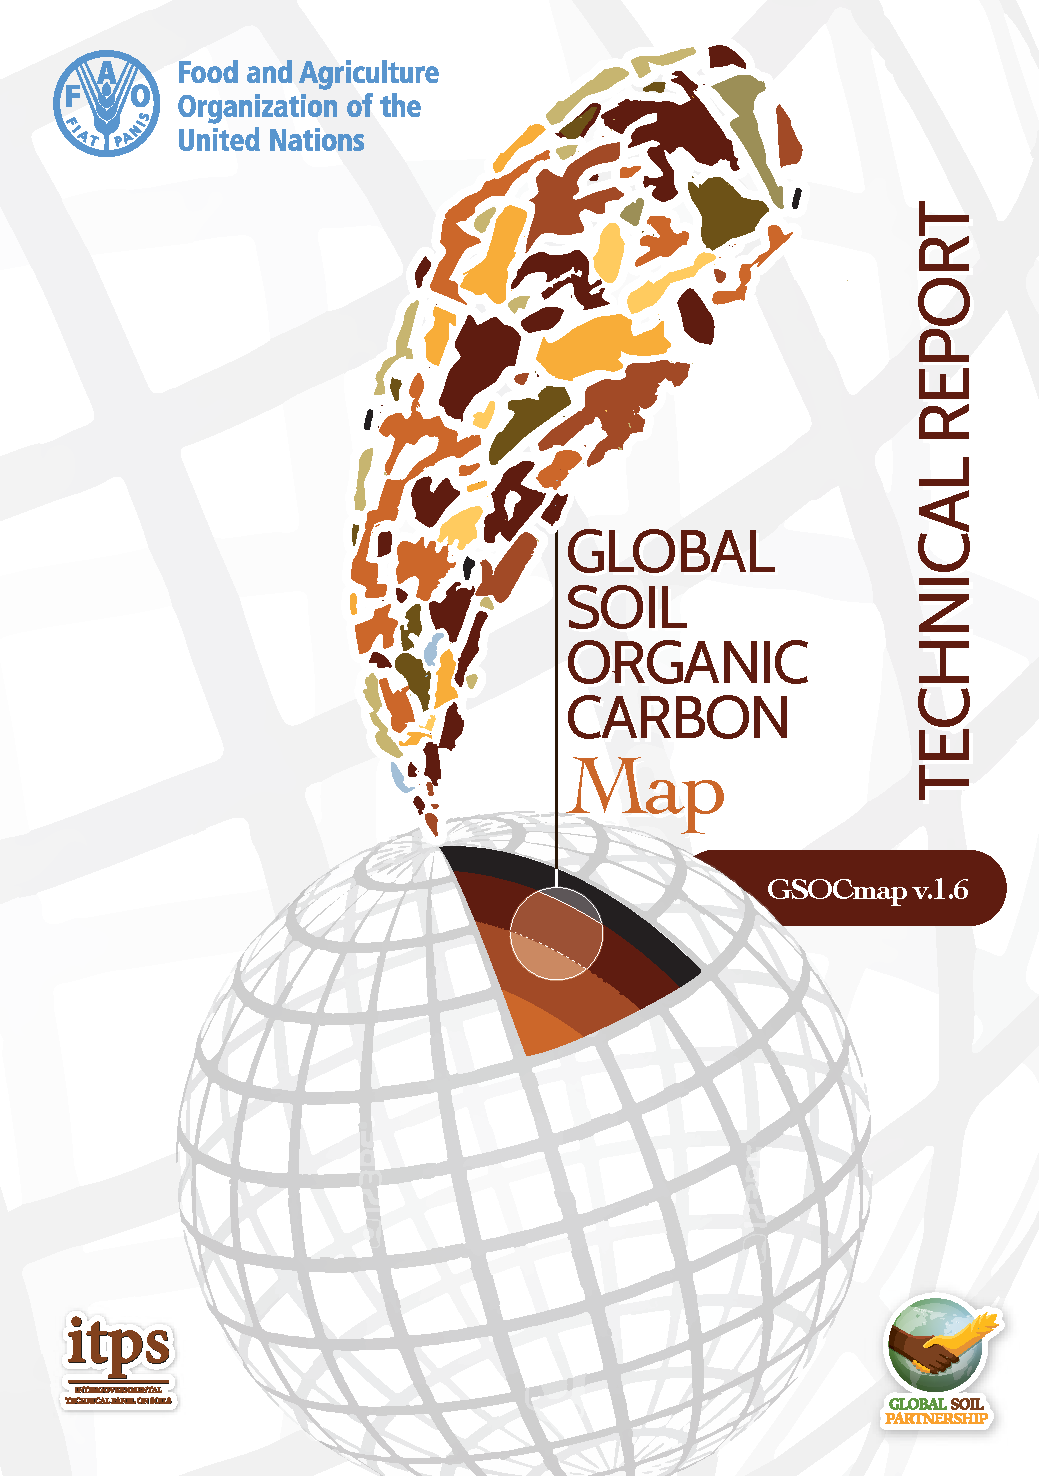
\includepdf{images/cover_1.6.pdf}
\afterpage{\blankpage}
\thispagestyle{empty}
\begin{titlepage}
    \begin{center}
        \vspace*{4cm}
        \Large

        \textcolor{astral}{\textbf{Country Guidelines on Digital Soil Mapping\\}}
        \vspace{0.5cm}
        \normalsize
        \vfill
        \noindent
        {\color{astral}\rule{\linewidth}{0.5mm} }

        Food and Agriculture Organization of the United Nations\\
	Rome, 2022
    \end{center}
\end{titlepage}
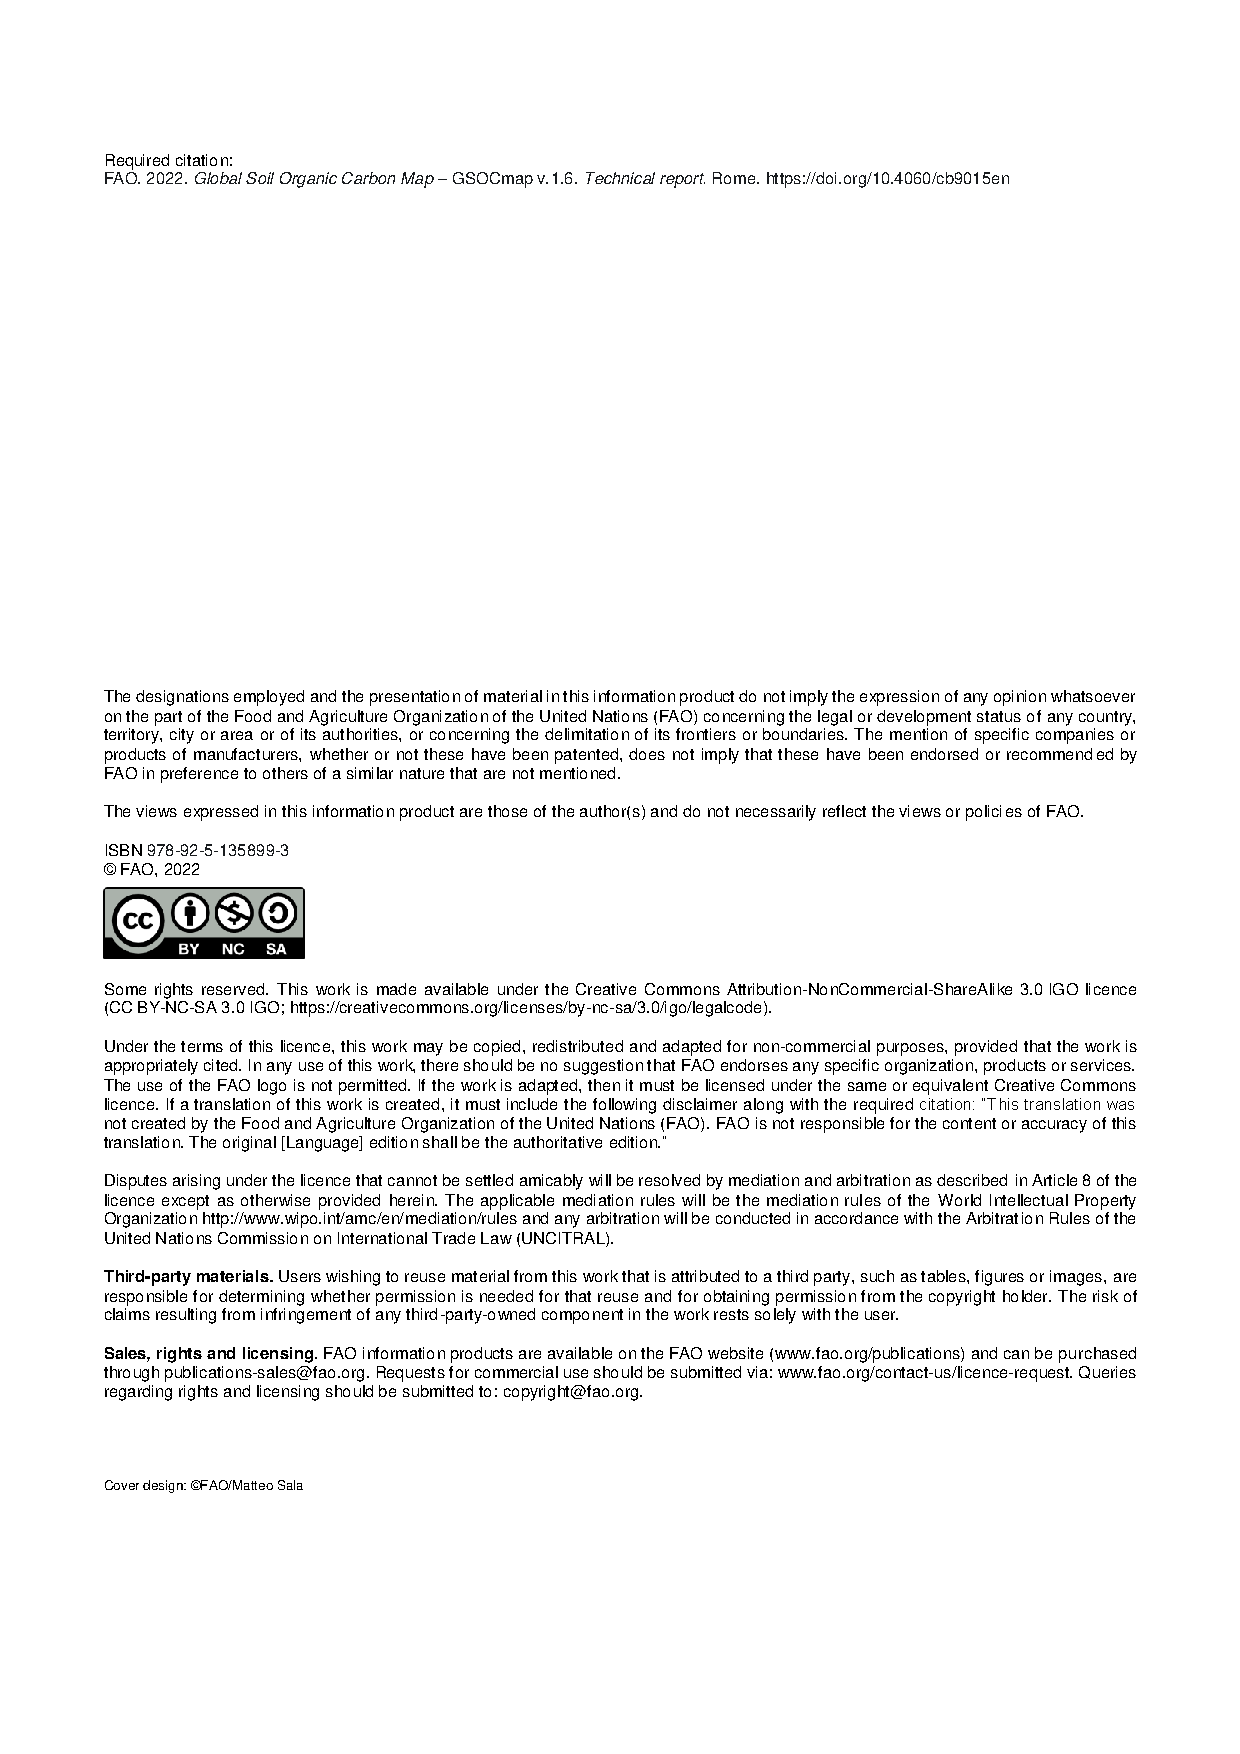
\includepdf{images/CB9015EN_Copyright Disclaimer_v2.pdf}


\frontmatter
\addtocontents{toc}{\protect\hypersetup{hidelinks}}   
\addtocontents{lof}{\protect\hypersetup{hidelinks}}
\addtocontents{lot}{\protect\hypersetup{hidelinks}}
\tableofcontents
\listoffigures
\listoftables
\nopagebreak[4]

\hypertarget{foreword}{%
\chapter*{Foreword}\label{foreword}}
\addcontentsline{toc}{chapter}{Foreword}

\hypertarget{abbreviations-and-acronyms}{%
\chapter*{Abbreviations and acronyms}\label{abbreviations-and-acronyms}}
\addcontentsline{toc}{chapter}{Abbreviations and acronyms}

\begin{description}
\item[BD]
Bulk Density
\item[CO\textsubscript{2}]
Carbon dioxide
\item[CRF]
Coarse fragments
\item[DM]
Dry matter
\item[DSM]
Digital soil mapping
\item[GAUL]
Global Administrative Unit Layers
\item[GHG]
Greenhouse gas
\item[GSOCmap]
Global Soil Organic Carbon Map
\item[GSOCseq]
Global Soil Organic Carbon Sequestration Potential Map
\item[GSP]
Global Soil Partnership
\item[HWSD]
Harmonized World Soil Database
\item[ISCN]
International Soil Carbon Network
\item[INSII]
International Network of Soil Information Institutions
\item[IPBES]
Intergovernmental Platform on Biodiversity and Ecosystem Services
\item[IPCC]
Intergovernmental Panel on Climate Change
\item[IPR]
Intellectual Property Rights
\item[ITPS]
Intergovernmental Technical Panel on Soils
\item[LDN]
Land Degradation Neutrality
\item[NDVI]
Normalized difference in vegetation index
\item[NPP]
Net Primary Production
\item[P4WG]
Pillar 4 Working Group
\item[QA/QC]
Quality Assurance/Quality Check
\item[RMSE]
Root mean square error
\item[SDF]
Soil Data Facility
\item[SDG]
Sustainable Development Goals
\item[SISLAC]
Latin America and the Caribbean's Soil Information System
\item[SOC]
Soil organic carbon
\item[SOM]
Soil organic matter
\item[SPADE/M]
Soil Profile Analytical Database of Europe of Measured Parameters
\item[SWRS]
Status of World's Soil Resources
\item[UNCCD]
United Nations Convention to Combat Desertification
\item[WFS]
Web Feature Service
\item[WoSIS]
World Soil Information Service
\end{description}

\hypertarget{contributors}{%
\chapter*{Contributors}\label{contributors}}
\addcontentsline{toc}{chapter}{Contributors}

\emph{Prepared by:}\\
\textbf{Global Soil Partnership Secretariat}\\
Guillermo Federico Olmedo\\
Kostiantyn Viatkin\\
Isabel Luotto\\
Moritz Mainka\\
Yusuf Yigini\\
Ronald Vargas\\
Mario Guevara Santamaría\\

\textbf{Second Intergovernmental Technical Panel on Soils}\\
Luca Montanarella - European Commission, Joint Research Centre
(\emph{Chair}); Saéb AbdelHaleem Khresat - Jordan; Isaurinda Dos Santos
Baptista Costa - Cape Verde; Sopon Chomchan -- Thailand; Juan Antonio
Comerma - Venezuela; Talal Darwish - Lebanon; Gunay Erpul - Turkey;
Fernando Garcia Préchac - Uruguay; Siosiua Halavatau - Tonga; Oneyda
Hernandez Lara - Cuba; Rainer Horn - Germany; Amanullah Khan - Pakistan;
Pavel Krasilnikov - Russia; Bhanooduth Lalljee - Mauritius; Botle
Mapeshoane - Lesotho; Neil McKenzie - Australia; Maria de Lourdes
Mendonca Santos -Brazil; Ahmad S. Muhaimeed - Iraq; Nsalambi V.
Nkongolo - Democratic Republic of the Congo; Brajendra Parmar - India;
Daniel John Pennock - Canada; Gary Pierzynski - USA; Peter de Ruiter -
The Netherlands; Miguel Taboada - Argentina; Kazuyuki Yagi -- Japan;
Martin Yemefack - Cameroon; Gan Lin Zhang -- China\\

\textbf{Third Intergovernmental Technical Panel on Soils}\\
Rosa Poch - Spain (\emph{Chair}); Nsalambi V. Nkongolo - Democratic Republic
of the Congo; Matshwene Edwin Moshia III - South Africa; Lydia Mumbi
Chabala - Zambia; Générose Nziguhueba - Burundi; Edmond Hien - Burkina
Faso; Ashok K. Patra - India; Jin Ke -- China; Chencho Norbu -- Bhutan;
Jun Murase - Japan; Mohammad Jamal Khan - Pakistan; Costanza Calzolari -
Italy; Ellen R. Graber - Israel; Peter de Ruiter - The Netherlands ;
Alexey Sorokin - Russian Federation; Adalberto Benavides Mendoza -
Mexico; Martha Marina Bolanos Benavides - Colombia; Fernando Garcia
Préchac - Uruguay; Lucía Helena Cunha dos Anjos - Brazil; Samuel Francke
Campana - Chile; Kutaiba M. Hassan - Iraq; Rafla Sahli Epse Attia -
Tunisia; Saéb AbdelHaleem Khresat - Jordan; Gary Pierzynski - USA; David
Allen Lobb - Canada; Siosiua Halavatau - Tonga; Megan Balks - New
Zealand\\

\mainmatter
\pagestyle{fancy}
\setlength{\headheight}{20.39996pt}

\hypertarget{background}{%
\chapter{Background}\label{background}}

\hypertarget{the-importance-of-soil-organic-carbon}{%
\section{The importance of soil organic carbon}\label{the-importance-of-soil-organic-carbon}}

\hypertarget{objectives-of-soil-organic-carbon-mapping}{%
\section{Objectives of soil organic carbon mapping}\label{objectives-of-soil-organic-carbon-mapping}}

This is a citation (\protect\hyperlink{ref-xie2015}{Xie, 2015}).

\hypertarget{data-policy}{%
\section{Data policy}\label{data-policy}}

\hypertarget{data-sharing-principles}{%
\subsection{Data sharing principles}\label{data-sharing-principles}}

The GSP Data Policy has been endorsed by partners of the Global Soil
Partnership during the 5th GSP Plenary Assembly in June 2017
(GSP \& FAO, 2017) in order to promote and govern soil data sharing for data
products including GSOCmap contributions, and considering harmonization
and interoperability requirements.\\
The GSP data policy aims to ensure that:

\begin{itemize}
\item
  every existing ownership right to shared soil data are respected;
\item
  the specific level of access and the conditions for data sharing are
  clearly specified;
\item
  the ownership of each dataset and web service are properly
  acknowledged and well-referenced; and
\item
  the data owners are protected from any liability arising from the
  use of their original and/or derived data.
\end{itemize}

It is recommended that data owners comply with the following open data
principles:

\begin{enumerate}
\def\labelenumi{\arabic{enumi}.}
\item
  Accessibility: the data shall be divulged through the Internet (web
  services).
\item
  Availability: the data is presented in a convenient,
  platform-independent, and in line with standard formats (e.g.~web
  feature service WFS).
\item
  License: the formal concession of the usage and access rights over
  the data shared.
\item
  Cost: data shall be shared free of cost, or at no more than a
  reasonable reproduction cost, preferably by downloading it from the
  Internet.
\item
  Re-use and Redistribution: data must be provided and licensed under
  terms that permit its reuse and redistribution, including
  intermixing with other datasets.
\item
  Global benefit: any user must be able to access, use and
  redistribute data of the Global Soil Information System. However,
  inherited restrictions by national data policies shall be accepted.
\item
  Metadata: data describing the products of the Global Soil
  Information System will by default be open for access.
\end{enumerate}

The data shared by the countries shall contain the relevant soil
information representative for the area portrayed. The shared datasets
contain the best available information for a given area and topic,
however, they are subject to potential restrictions based on the
institutions' or countries' data policy.\\
The data shared by the countries should be quality controlled which
means that the data have been technically evaluated to ensure data
integrity, correctness, and completeness; errors and omissions are
identified and, if possible, addressed.\\

\hypertarget{ownership-data-rights-and-citation}{%
\subsection{Ownership, data rights and citation}\label{ownership-data-rights-and-citation}}

In the case of original data, the rightful data owner keeps full
ownership of it. All intellectual property rights (IPR) and copyrights
pertaining to the data owner remain intact and are respected by the soil
data facility (SDF) host. All data providers must communicate to the SDI
host their IPR and data use policies. Thus, the ownership of all data
made available through the GSP soil portal need to be clearly specified.
This is an important prerequisite to allow this data to be accessible
through the soil SDF.\\
In the case of derived data, the deriving institution becomes the
rightful owner. However, all original data must be accredited and
correctly cited. According to the Pillar 4 Implementation Plan, each
global-level derived GSP data product will be quality-assured by the
Pillar 4 Working Group. This includes agreements about the correct
citation.\\
The data owner shall ensure that the data shared can be used and
interpreted by the authorized users in general; this includes providing
the proper citations, as well as providing information over the
ownership of such data for acknowledgement purposes. Users shall
acknowledge the source of data provided through the Global Soil
Information System.\\
All providers of original data (data owners) are responsible to define
and clarify the IPR and licensing. Any user of this data, such as the
SDF host, has to respect the national data policies and/or licensing
involved with the retrieval of the respective web services. In the case
of data provided to the central repository, a bilateral
agreement/license may be required (between the national data owner and
SDF host), depending on and in conformity with national rules.\\
More information about the data policy can be accessed at GSP \& FAO (2017).

\hypertarget{setting-up-the-software-environment}{%
\chapter{Setting-up the software environment}\label{setting-up-the-software-environment}}

\emph{Y. Yigini}

This cookbook focuses on SOC modeling using open source digital mapping tools. The instructions in this chapter will guide user through installing and manually configuring the software to be used for DSM procedures for Microsoft Windows desktop platform. Instructions for the other platforms (e.g.~Linux Flavours, MacOS) can be found through free online resources.

\hypertarget{use-of-r-rstudio-and-r-packages}{%
\section{Use of R, RStudio and R Packages}\label{use-of-r-rstudio-and-r-packages}}

\textbf{R} is a language and environment for statistical computing. It provides a wide variety of statistical (e.g.~linear modeling, statistical tests, time-series, classification, clustering, etc.) and graphical methods, and is highly extensible.

\hypertarget{obtaining-and-installing-r}{%
\subsection{Obtaining and installing R}\label{obtaining-and-installing-r}}

Installation files and instructions can be downloaded from the Comprehensive R Archive Network (CRAN).

\begin{enumerate}
\def\labelenumi{\arabic{enumi}.}
\tightlist
\item
  Go to the following link \url{https://cloud.r-project.org/index.html} to download and install \textbf{R}.
\item
  Pick an installation file for your platform.
\end{enumerate}

\hypertarget{obtaining-and-installing-rstudio}{%
\subsection{Obtaining and installing RStudio}\label{obtaining-and-installing-rstudio}}

Beginners will find it very hard to start using \textbf{R} because it has no Graphical User Interface (GUI). There are some GUIs which offer some of the functionality of \textbf{R}. \textbf{RStudio} makes \textbf{R} easier to use. It includes a code editor, debugging and visualization tools. Similar steps need to be followed to install \textbf{RStudio}.

\begin{enumerate}
\def\labelenumi{\arabic{enumi}.}
\tightlist
\item
  Go to \url{https://www.rstudio.com/products/rstudio/download/} to download and install \textbf{RStudio}'s open source edition.
\item
  On the download page, \emph{RStudio Desktop, Open Source License} option should be selected.
\item
  Pick an installation file for your platform.
\end{enumerate}

\hypertarget{getting-started-with-r}{%
\subsection{Getting started with R}\label{getting-started-with-r}}

\begin{itemize}
\tightlist
\item
  \textbf{R} manuals: \url{http://cran.r-project.org/manuals.html}
\item
  Contributed documentation: \url{http://cran.r-project.org/other-docs.html}
\item
  Quick-\textbf{R}: \url{http://www.statmethods.net/index.html}
\item
  Stackoverflow \textbf{R} community: \url{https://stackoverflow.com/questions/tagged/r}
\end{itemize}

\hypertarget{r-packages}{%
\section{R packages}\label{r-packages}}

When you download \textbf{R}, you get the basic \textbf{R} system which implements the \textbf{R} language. \textbf{R} becomes more useful with the large collection of packages that extend the basic functionality of it. \textbf{R} packages are developed by the \textbf{R} community.

\hypertarget{finding-r-packages}{%
\subsection{Finding R packages}\label{finding-r-packages}}

The primary source for \textbf{R} packages is \href{https://cran.r-project.org/}{CRAN's} official website, where currently about 12,000 available packages are listed. For spatial applications, various packages are available. You can obtain information about the available packages directly on CRAN with the \texttt{available.packages()} function. The function returns a matrix of details corresponding to packages currently available at one or more repositories. An easier way to browse the list of packages is using the \href{https://cran.r-project.org/web/views/}{\emph{Task Views}} link, which groups together packages related to a given topic.

\hypertarget{most-used-r-packages-for-digital-soil-mapping}{%
\subsection{Most used R packages for digital soil mapping}\label{most-used-r-packages-for-digital-soil-mapping}}

As was previously mentioned, \textbf{R} is extensible through packages. \textbf{R} packages are collections of \textbf{R} functions, data, documentation and compiled code easy to share with others. In the following Subsections, we are going to present the most used packages related to digital soil property mapping.

\hypertarget{SoilPedometrics}{%
\subsubsection{Soil science and pedometrics}\label{SoilPedometrics}}

\href{https://CRAN.R-project.org/package=aqp}{\textbf{aqp}}: Algorithms for quantitative pedology. A collection of algorithms related to modeling of soil resources, soil classification, soil profile aggregation, and visualization.

\href{https://CRAN.R-project.org/package=GSIF}{\textbf{GSIF}}: Global Soil Information Facility (GSIF). Tools, functions and sample datasets for digital soil mapping. GSIF tools (standards and functions) and sample datasets for global soil mapping.

\href{http://ithir.r-forge.r-project.org/}{\textbf{ithir}}: A collection of functions and algorithms specific to pedometrics. The package was developed by Brendan Malone at the University of Sydney.

\href{https://CRAN.R-project.org/package=soiltexture}{\textbf{soiltexture}}: The \href{https://cran.r-project.org/web/packages/soiltexture/vignettes/soiltexture_vignette.pdf}{\emph{Soil Texture Wizard}} is a set of \textbf{R} functions designed to produce texture triangles (also called texture plots, texture diagrams, texture ternary plots), classify and transform soil textures data. These functions virtually allow to plot any soil texture triangle (classification) into any triangle geometry (isosceles, right-angled triangles, etc.). The set of functions is expected to be useful to people using soil textures data from different soil texture classification or different particle size systems. Many (\textgreater{} 15) texture triangles from all around the world are predefined in the package. A simple text-based GUI is provided: \texttt{soiltexture\_gui()}.

\hypertarget{spatial-analysis}{%
\subsubsection{Spatial analysis}\label{spatial-analysis}}

\href{https://CRAN.R-project.org/package=raster}{\textbf{raster}}: Reading, writing, manipulating, analyzing and modeling of gridded spatial data. The package implements basic and high-level functions, processing of very large files is supported.

\href{https://CRAN.R-project.org/package=rgdal}{\textbf{rgdal}}: Provides bindings to Frank Warmerdam's Geospatial Data Abstraction Library (GDAL).

\href{https://CRAN.R-project.org/package=RSAGA}{\textbf{RSAGA}}: The package provides access to geocomputing and terrain analysis functions of \href{/url\%7Bhttp://www.saga-gis.org/en/index.html\%7D}{SAGA GIS} from within \textbf{R} by running the command line version of System for Automated Geoscientific Analyses (SAGA).

\href{https://cran.r-project.org/web/packages/sf/index.html}{\textbf{sf}}: The package provides an improvement on \textbf{sp} and \textbf{rgdal} for spatial datasets. It is using the newly Simple Feratures (SF) standard which is widely implemented in spatial databases (PostGIS, ESRI ArcGIS), and forms the vector data basis for libraries such as GDAL and web standards such as GeoJSON (\url{http://geojson.org/}).

\href{https://CRAN.R-project.org/package=sp}{\textbf{sp}}: The package provides classes and methods for spatial data. The classes document where the spatial location information resides, for 2D or 3D data.

\hypertarget{modelling}{%
\subsubsection{Modelling}\label{modelling}}

\href{https://CRAN.R-project.org/package=automap}{\textbf{automap}}: This package performs an automatic interpolation by automatically estimating the variogram and then calling \href{https://CRAN.R-project.org/package=gstat}{\textbf{gstat}}.

\href{https://CRAN.R-project.org/package=caret}{\textbf{caret}}: Extensive range of functions for training and plotting classification and regression models.

\href{https://CRAN.R-project.org/package=Cubist}{\textbf{Cubist}}: Regression modeling using rules with added instance-based corrections. Cubist models were developed by Ross Quinlan.

\href{https://CRAN.R-project.org/package=C5.0}{\textbf{C5.0}}: C5.0 decision trees and rule-based models for pattern recognition. Another model structure developed by Ross Quinlan.

\href{https://CRAN.R-project.org/package=gam}{\textbf{gam}}: Functions for fitting and working with generalized additive models.

\href{https://CRAN.R-project.org/package=gstat}{\textbf{gstat}}: Variogram modeling with simple, ordinary and universal point or block (co)kriging, sequential Gaussian or indicator (co)simulation. The package includes variogram and variogram map plotting utility functions.

\href{https://CRAN.R-project.org/package=nnet}{\textbf{nnet}}: Software for feed-forward neural networks with a single hidden layer, and for multinomial log-linear models.

\hypertarget{mapping-and-plotting}{%
\subsubsection{Mapping and plotting}\label{mapping-and-plotting}}

Both \textbf{raster} and \textbf{sp} have handy functions for plotting spatial data. The following packages can be used as functional extentions.

\href{https://cran.r-project.org/web/packages/ggplot2/index.html}{\textbf{ggplot2}}: Besides using the base plotting functionality, this is another useful plotting package.

\href{https://CRAN.R-project.org/package=leaflet}{\textbf{leaflet}}: Create and customize interactive maps using the Leaflet JavaScript library and the \href{https://cran.r-project.org/web/packages/htmlwidgets/index.html}{\textbf{htmlwidgets}} package. These maps can be used directly from the \textbf{R} console, from \textbf{RStudio}, in \href{https://shiny.rstudio.com/}{\textbf{Shiny}} apps and \textbf{RMarkdown} documents.

\href{https://CRAN.R-project.org/package=plotKML}{\textbf{plotKML}}: Writes sp-class, spacetime-class, raster-class and similar spatial and spatiotemporal objects to KML following some basic cartographic rules.

\hypertarget{packages-used-in-this-cookbook}{%
\subsection{Packages used in this cookbook}\label{packages-used-in-this-cookbook}}

The authors of this cookbook used a number of different \textbf{R} packages. All required packages used in the cookbook can be installed using the following code and the \texttt{install.packages()} function when starting a new SOC mapping project. Alternatively, the code for the installation of the needed packages is included at the beginning of each Chapter.

\begin{Shaded}
\begin{Highlighting}[]
\CommentTok{\# Install all required R packages used in the cookbook}
\FunctionTok{install.packages}\NormalTok{(}\FunctionTok{c}\NormalTok{(}\StringTok{"aqp"}\NormalTok{, }\StringTok{"automap"}\NormalTok{, }\StringTok{"car"}\NormalTok{, }\StringTok{"caret"}\NormalTok{, }\StringTok{"e1071"}\NormalTok{,}
                   \StringTok{"GSIF"}\NormalTok{, }\StringTok{"htmlwidgets"}\NormalTok{, }\StringTok{"leaflet"}\NormalTok{, }\StringTok{"mapview"}\NormalTok{,}
                   \StringTok{"Metrics"}\NormalTok{, }\StringTok{"openair"}\NormalTok{, }\StringTok{"plotKML"}\NormalTok{, }\StringTok{"psych"}\NormalTok{, }
                   \StringTok{"quantregForest"}\NormalTok{, }\StringTok{"randomForest"}\NormalTok{, }\StringTok{"raster"}\NormalTok{,}
                   \StringTok{"rasterVis"}\NormalTok{, }\StringTok{"reshape"}\NormalTok{, }\StringTok{"rgdal"}\NormalTok{, }\StringTok{"RSQLite"}\NormalTok{,}
                   \StringTok{"snow"}\NormalTok{, }\StringTok{"soiltexture"}\NormalTok{, }\StringTok{"sf"}\NormalTok{, }\StringTok{"sp"}\NormalTok{))}
\end{Highlighting}
\end{Shaded}

\hypertarget{r-and-spatial-data}{%
\section{R and spatial data}\label{r-and-spatial-data}}

\textbf{R} has a large and growing number of spatial data packages. We recommend taking a quick browse on \textbf{R}'s official website to see the spatial packages available: \url{http://cran.r-project.org/web/views/Spatial.html}.

\hypertarget{reading-shapefiles}{%
\subsection{Reading shapefiles}\label{reading-shapefiles}}

The Environmental Systems Research Institute (ESRI) provides a shapefile format SHP which is widely used for storing vector-based spatial data (i.e., points, lines, polygons). This example demonstrates use of \textbf{raster} package that provides functions for reading and/or writing shapefiles.

\begin{Shaded}
\begin{Highlighting}[]
\FunctionTok{library}\NormalTok{(raster)}
\CommentTok{\# Load the soil map from a shapefile *.shp file}
\NormalTok{soilmap }\OtherTok{\textless{}{-}} \FunctionTok{shapefile}\NormalTok{(}\StringTok{"MK\_soilmap\_simple.shp"}\NormalTok{)}
\end{Highlighting}
\end{Shaded}

We may want to use these data in other GIS environments such as ArcGIS, QGIS, SAGA GIS, etc. This means we need to export the \texttt{SpatialPointsDataFrame} to an appropriate spatial data format such as a shapefile \texttt{*.shp}.

\begin{Shaded}
\begin{Highlighting}[]
\CommentTok{\# For example, we can select the soil units classified as }
\CommentTok{\# fluvisols according to WRB}
\NormalTok{Fluvisols }\OtherTok{\textless{}{-}}\NormalTok{ soilmap[soilmap}\SpecialCharTok{$}\NormalTok{WRB }\SpecialCharTok{==} \StringTok{"Fluvisol"}\NormalTok{,]}

\CommentTok{\# Save this as a new shapefile }
\FunctionTok{shapefile}\NormalTok{(Fluvisols, }\AttributeTok{filename =} \StringTok{\textquotesingle{}results/fluvisols.shp\textquotesingle{}}\NormalTok{,}
          \AttributeTok{overwrite =} \ConstantTok{TRUE}\NormalTok{)}
\end{Highlighting}
\end{Shaded}

\hypertarget{coordinate-reference-systems-in-r}{%
\subsection{Coordinate reference systems in R}\label{coordinate-reference-systems-in-r}}

We need to define the Coordinate Reference System (CRS) to be able to perform any sort of spatial analysis in \textbf{R}. To clearly tell \textbf{R} this information we define the CRS which describes a reference system in a way understood by the PROJ.4 projection library. Find more information at this link: \url{http://trac.osgeo.org/proj/}.

An interface to the PROJ.4 library is available in the \textbf{rgdal} package. An alternative to using PROJ.4 character strings, we can use the corresponding yet simpler EPSG (European Petroleum Survey Group) code. \textbf{rgdal} also recognizes these codes. If you are unsure of the PROJ.4 or EPSG code for the spatial data that you have but know the CRS, you should consult \url{http://spatialreference.org/} for assistance.

\begin{Shaded}
\begin{Highlighting}[]
\CommentTok{\# Print the CRS for the object soilmap}
\NormalTok{soilmap}\SpecialCharTok{@}\NormalTok{proj4string}
\end{Highlighting}
\end{Shaded}

The following example shows how a spatial object from a (comma-separated values) CSV file (\texttt{*.csv}) can be created. We can use the \texttt{coordinates()} function from the \textbf{sp} package to define which columns in the data frame refer to actual spatial coordinates. Here, the coordinates are listed in columns X and Y.

\begin{Shaded}
\begin{Highlighting}[]
\CommentTok{\# Load the table with the soil observations site information}
\NormalTok{dat\_sites }\OtherTok{\textless{}{-}} \FunctionTok{read.csv}\NormalTok{(}\AttributeTok{file =} \StringTok{"data/site{-}level.csv"}\NormalTok{)}

\CommentTok{\# Convert from table to spatial points object}
\FunctionTok{coordinates}\NormalTok{(dat\_sites) }\OtherTok{\textless{}{-}} \ErrorTok{\textasciitilde{}}\NormalTok{ X }\SpecialCharTok{+}\NormalTok{ Y}

\CommentTok{\# Check the coordinate system}
\NormalTok{dat\_sites}\SpecialCharTok{@}\NormalTok{proj4string}

\CommentTok{\# As the CRS is not defined, we can assign the correct CRS as we}
\CommentTok{\# have information about it. In this case, it should be EPSG:4326}
\NormalTok{dat\_sites}\SpecialCharTok{@}\NormalTok{proj4string }\OtherTok{\textless{}{-}} \FunctionTok{CRS}\NormalTok{(}\StringTok{"+init=epsg:4326"}\NormalTok{)}

\CommentTok{\# Check the CRS again}
\NormalTok{dat\_sites}\SpecialCharTok{@}\NormalTok{proj4string}
\end{Highlighting}
\end{Shaded}

\hypertarget{working-with-rasters}{%
\subsection{Working with rasters}\label{working-with-rasters}}

Most of the functions for handling raster data are available in the \textbf{raster} package. There are functions for reading and writing raster files from and to different formats. In DSM, we mostly work with data in table format and then rasterize this data so that we can produce a continuous map. For doing this in \textbf{R} environment, we will load raster data in a data frame. This data is a digital elevation model (DEM) provided by the International Soil Reference and Information Centre (ISRIC) for FYROM.

\begin{Shaded}
\begin{Highlighting}[]
\CommentTok{\# For handling raster data, we load raster package}
\FunctionTok{library}\NormalTok{(raster)}

\CommentTok{\# Load DEM from the raster *.tif files}
\NormalTok{DEM }\OtherTok{\textless{}{-}} \FunctionTok{raster}\NormalTok{(}\StringTok{"covs/DEMENV5.tif"}\NormalTok{)}
\end{Highlighting}
\end{Shaded}

We may want to export this raster to a suitable format to work in a standard GIS environment. See the help file for writing a raster \texttt{?writeRaster} to get information regarding the supported grid types that data can be exported into. Here, we will export our raster to ESRI ASCII (American Standard Code for Information Interchange), as it is a common and universal raster format.

We may also want to export our DEM to KML (Keyhole Markup Language) file (\texttt{*.kml}) using the \texttt{KML()} function. \texttt{KML()} is a handy function from the \textbf{raster} package for exporting grids to KML format. Note that we need to re-project the data to the World Geodetic System (WGS) WGS84 geographic. The raster re-projection is performed using the \texttt{projectRaster()} function. Look at the help file \texttt{?projectRaster} for more information.

\hypertarget{other-dsm-software-and-tools}{%
\section{Other DSM software and tools}\label{other-dsm-software-and-tools}}

\begin{itemize}
\tightlist
\item
  \textbf{GRASS GIS}: Available at \url{https://grass.osgeo.org/} (free and open source).
\item
  \textbf{SAGA GIS}: Available at \url{https://sourceforge.net/projects/saga-gis/files/} (free and open source).
\item
  \textbf{QGIS}: Available at \url{http://www.qgis.org/en/site/forusers/download.html} (free and open source).
\end{itemize}

\hypertarget{product-specifications}{%
\chapter{Product specifications}\label{product-specifications}}

\hypertarget{generic-target-specification}{%
\section{Generic target specification}\label{generic-target-specification}}

\hypertarget{metadata-specifications}{%
\section{Metadata specifications}\label{metadata-specifications}}

\hypertarget{data-collection-and-processing}{%
\chapter{Data collection and processing}\label{data-collection-and-processing}}

\hypertarget{different-scenarios-of-country-driven-action}{%
\section{Different scenarios of country driven action}\label{different-scenarios-of-country-driven-action}}

\hypertarget{delivery-of-the-maps-produced-by-the-countries}{%
\subsection{Delivery of the maps produced by the countries}\label{delivery-of-the-maps-produced-by-the-countries}}

\hypertarget{data-submission-form}{%
\subsubsection{Data submission form}\label{data-submission-form}}

\hypertarget{joint-efforts}{%
\subsection{Joint efforts}\label{joint-efforts}}

\hypertarget{gsp-gapfilling}{%
\subsection{GSP gapfilling}\label{gsp-gapfilling}}

\hypertarget{spatial-modeling-using-publicly-available-data}{%
\subsubsection{Spatial modeling using publicly available data}\label{spatial-modeling-using-publicly-available-data}}

\hypertarget{using-publicly-available-soc-stock-maps}{%
\subsubsection{Using publicly available SOC stock maps}\label{using-publicly-available-soc-stock-maps}}

\hypertarget{data-processing-and-compilation-of-the-gsocmap}{%
\section{Data processing and compilation of the GSOCmap}\label{data-processing-and-compilation-of-the-gsocmap}}

\hypertarget{blocks}{%
\chapter{Blocks}\label{blocks}}

\hypertarget{equations}{%
\section{Equations}\label{equations}}

Here is an equation.

\begin{equation} 
  f\left(k\right) = \binom{n}{k} p^k\left(1-p\right)^{n-k}
  \label{eq:binom}
\end{equation}

You may refer to using \texttt{\textbackslash{}@ref(eq:binom)}, like see Equation \eqref{eq:binom}.

\hypertarget{theorems-and-proofs}{%
\section{Theorems and proofs}\label{theorems-and-proofs}}

Labeled theorems can be referenced in text using \texttt{\textbackslash{}@ref(thm:tri)}, for example, check out this smart theorem \ref{thm:tri}.

\begin{theorem}
\protect\hypertarget{thm:tri}{}\label{thm:tri}For a right triangle, if \(c\) denotes the \emph{length} of the hypotenuse
and \(a\) and \(b\) denote the lengths of the \textbf{other} two sides, we have
\[a^2 + b^2 = c^2\]
\end{theorem}

Read more here \url{https://bookdown.org/yihui/bookdown/markdown-extensions-by-bookdown.html}.

\hypertarget{callout-blocks}{%
\section{Callout blocks}\label{callout-blocks}}

The R Markdown Cookbook provides more help on how to use custom blocks to design your own callouts: \url{https://bookdown.org/yihui/rmarkdown-cookbook/custom-blocks.html}

\hypertarget{blocks-1}{%
\chapter{Blocks}\label{blocks-1}}

\hypertarget{equations-1}{%
\section{Equations}\label{equations-1}}

Here is an equation.

\begin{equation} 
  f\left(k\right) = \binom{n}{k} p^k\left(1-p\right)^{n-k}
  \label{eq:binom}
\end{equation}

You may refer to using \texttt{\textbackslash{}@ref(eq:binom)}, like see Equation \eqref{eq:binom}.

\hypertarget{theorems-and-proofs-1}{%
\section{Theorems and proofs}\label{theorems-and-proofs-1}}

Labeled theorems can be referenced in text using \texttt{\textbackslash{}@ref(thm:tri)}, for example, check out this smart theorem \ref{thm:tri}.

\begin{theorem}
\protect\hypertarget{thm:tri}{}\label{thm:tri}For a right triangle, if \(c\) denotes the \emph{length} of the hypotenuse
and \(a\) and \(b\) denote the lengths of the \textbf{other} two sides, we have
\[a^2 + b^2 = c^2\]
\end{theorem}

Read more here \url{https://bookdown.org/yihui/bookdown/markdown-extensions-by-bookdown.html}.

\hypertarget{callout-blocks-1}{%
\section{Callout blocks}\label{callout-blocks-1}}

The R Markdown Cookbook provides more help on how to use custom blocks to design your own callouts: \url{https://bookdown.org/yihui/rmarkdown-cookbook/custom-blocks.html}

\hypertarget{blocks-2}{%
\chapter{Blocks}\label{blocks-2}}

\hypertarget{equations-2}{%
\section{Equations}\label{equations-2}}

Here is an equation.

\begin{equation} 
  f\left(k\right) = \binom{n}{k} p^k\left(1-p\right)^{n-k}
  \label{eq:binom}
\end{equation}

You may refer to using \texttt{\textbackslash{}@ref(eq:binom)}, like see Equation \eqref{eq:binom}.

\hypertarget{theorems-and-proofs-2}{%
\section{Theorems and proofs}\label{theorems-and-proofs-2}}

Labeled theorems can be referenced in text using \texttt{\textbackslash{}@ref(thm:tri)}, for example, check out this smart theorem \ref{thm:tri}.

\begin{theorem}
\protect\hypertarget{thm:tri}{}\label{thm:tri}For a right triangle, if \(c\) denotes the \emph{length} of the hypotenuse
and \(a\) and \(b\) denote the lengths of the \textbf{other} two sides, we have
\[a^2 + b^2 = c^2\]
\end{theorem}

Read more here \url{https://bookdown.org/yihui/bookdown/markdown-extensions-by-bookdown.html}.

\hypertarget{callout-blocks-2}{%
\section{Callout blocks}\label{callout-blocks-2}}

The R Markdown Cookbook provides more help on how to use custom blocks to design your own callouts: \url{https://bookdown.org/yihui/rmarkdown-cookbook/custom-blocks.html}

\hypertarget{references}{%
\chapter*{References}\label{references}}
\addcontentsline{toc}{chapter}{References}

\hypertarget{refs}{}
\begin{CSLReferences}{0}{0}
\leavevmode\hypertarget{ref-xie2015}{}%
\textbf{Xie, Y.} 2015. \emph{Dynamic documents with {R} and knitr}. 2nd edition. Boca Raton, Florida, Chapman; Hall/CRC. (also available at \url{http://yihui.org/knitr/}).

\end{CSLReferences}

%\printindex
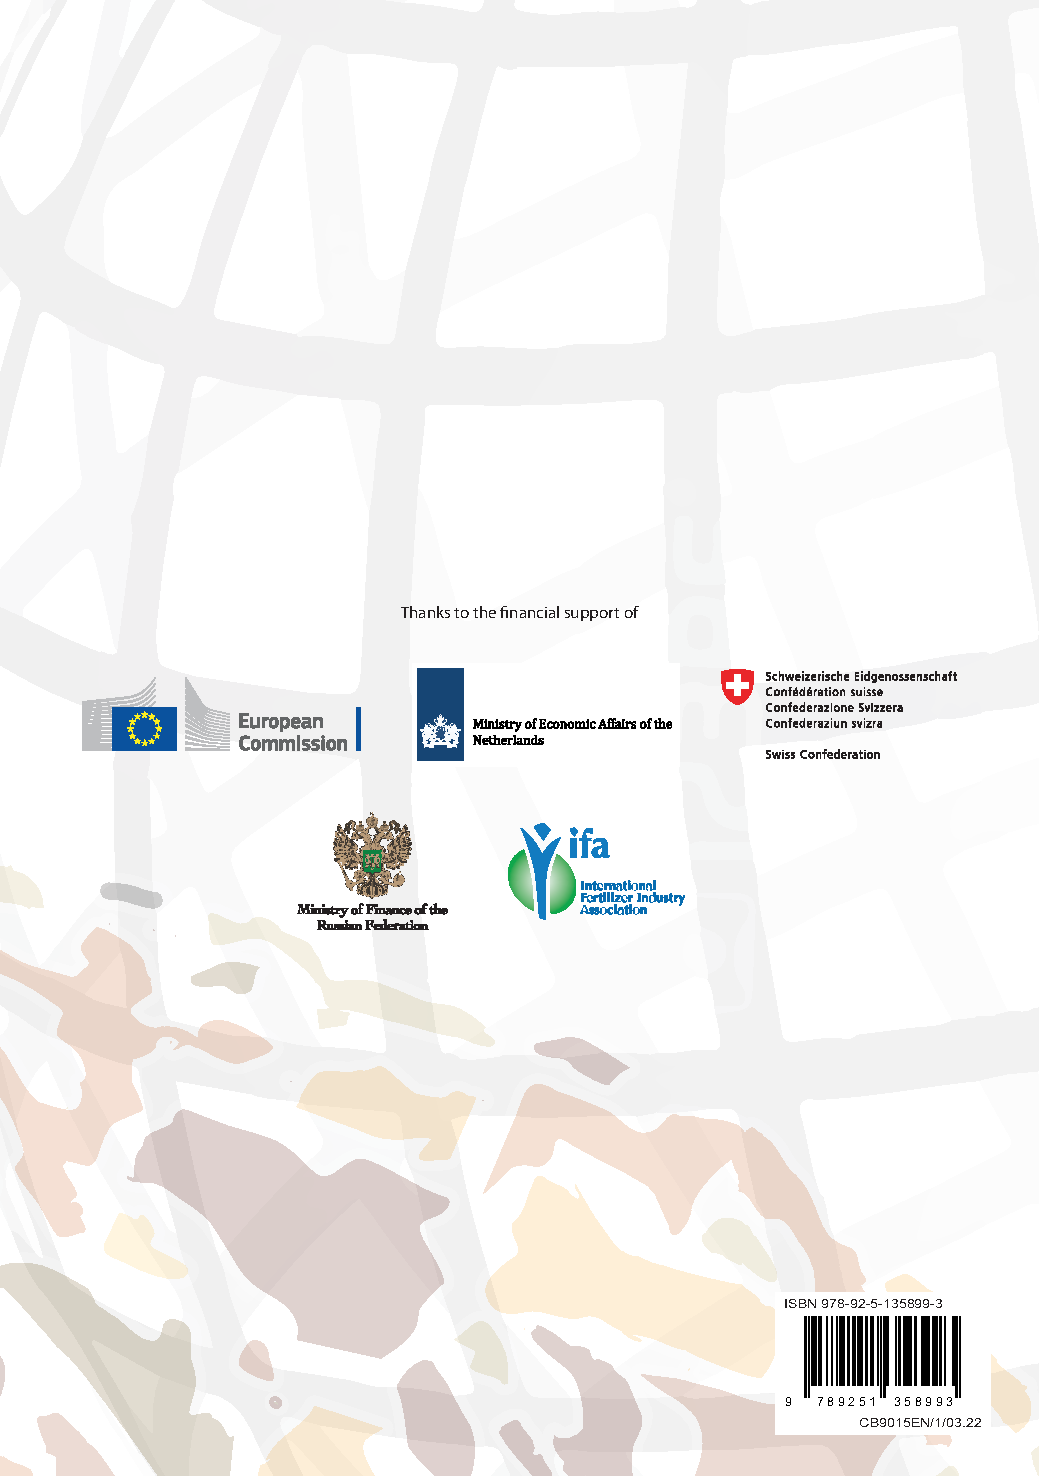
\includepdf{images/backcover.pdf}

\end{document}
